% ============================================================================
%  s05-examples.tex —— 第 5 节「例子」
%  原文：Ivan Smith, A Symplectic Prolegomenon, arXiv:1401.0269v2
%  对应源码：p0269/src/Prolegomenon_utf8.tex 第 1369--1494 行
% ============================================================================

\section{例子}\label{Sec:Examples}

\begin{keypoints}
\begin{itemize}
  \item \textbf{核心图像}：本节以一批可以“显式”计算的流形，说明 Fukaya 范畴的生成元与显式代数模型：二维环面、亏格 2 曲面、四维环面、偶维二次超曲面、环簇 Fano 簇与四次 K3 曲面。
  \item \textbf{关键工具}：球状对象的生成判据（命题 \ref{Prop:SpheresGenerate}）、Lefschetz 纤维化与扭曲复形、道路代数的 $A_{\infty}$-结构、quilt 型 Künneth 定理、pearl 模型与谱序列。
  \item \textbf{结论}：这些例子的导出 Fukaya 范畴分别等价于椭圆曲线上的凝聚层、$E\times E$ 上的凝聚层、显式 $A_{\infty}$-代数上的模等代数对象；反过来，范畴计算也给出辛拓扑结论（例如四维环面上辛同胚的不动点下界）。
  \item \textbf{与前后文的联系}：本节把前文的生成判据与 $A_\infty$ 代数工具落到实处，并为第 6 节的稳定性条件与 Orlov 谱提供计算素材。
\end{itemize}
\end{keypoints}

我们“显式地”描述若干流形的 Fukaya 范畴。这些例子是实曲面（其上的拉格朗日圆圈不界定任何圆盘）、Calabi--Yau 曲面（由例 \ref{Ex:CY} 所支配）或单调簇，因此这些范畴可以用初等手段定义。

\subsection{二维环面} 取 $\bK = \Lambda$。应用命题 \ref{Prop:SpheresGenerate} 可知，经圈 $l$ 与子午圈 $m$ 分裂生成 $\scrF(T^2)$。事实上，$(\tau_l \tau_m)^6 = \id$，相应的 Lefschetz 纤维化 $\scrX \rightarrow \bP^1$ 是有理椭圆曲面，而圈类 $\mathcal{C}(w)$ 计数有限多条 $(-1)$-曲线截面，故其取值是 $H^2(T^2)$ 中最高类的非零倍数。圆圈 $l$、$m$ 不界定任何全纯圆盘，故其自 Floer 上同调等于 $H^*(S^1)$。两圆横截相交于唯一一点，这给出生成元 $[p]\in HF^0(l,m)$ 与 $[q]\in HF^1(m,l)$。这里 $p$ 的分次是选定的，而 $q$ 的分次由 Poincaré 对偶强制决定；后者同时蕴含乘积 $\mu^2(p,q)$ 与 $\mu^2(q,p)$ 非平凡。由分次理由，除幺性所强制的乘积之外，这些就是全部非平凡乘积。

% [Tutor Note: $(\tau_l\tau_m)^6=\id$ 即椭圆纤维化的辫关系，是模群 $SL(2,\bZ)$ 中“双曲”元素的阶；它是把 $T^2$ 的 Lefschetz 纤维化实现为有理椭圆曲面的关键。核对时注意 $\tau_l,\tau_m$ 为沿 $l,m$ 的正 Dehn 扭转，方向或符号约定相反时会得到 $(\tau_l\tau_m)^{-6}$，但不影响本段论证。]

由此可知，六维代数 $A = HF(l \oplus m, l \oplus m)$ 可以描述为下图箭图 $Q$ 的道路代数 $\Pi\,Q$ 的商
\begin{equation*}
\xymatrix{
 l \ \ar@/^/^{[p]}[r] & \ m\ar@/^/^{[q]}[l]
}
\end{equation*}
模去由合成 $a\rightarrow b\rightarrow a \rightarrow b$ 与 $b\rightarrow a \rightarrow b \rightarrow a$ 生成的理想，亦即 $\Pi\,Q / \langle J\rangle^3$，其中 $J$ 为所有箭头生成的理想。对于道路代数模去箭头理想的幂所得的商，bar 复形含有大量零调子复形，这意味着 Hochschild 上同调可以相当容易地计算。

从这里出发，Lekili 与 Perutz \cite{LekiliPerutz} 确定了六维代数 $A$ 上所有可能的 $A_{\infty}$-结构。

% [Tutor Note: 作者说“bar 复形含大量零调子复形”而未给证明；其要点是：模去箭头理想的高次幂后，商代数在道路长度滤过下的各项是半单的，于是 Hochschild 链复形可按滤过逐层用标准的条复形（bar/Koszul）论证消去。具体计算建议先分别处理 $J^2$ 与 $J^3$ 两层，再核对乘法 $\mu^2$ 的复合是否恰落入 $\langle J\rangle^3$。]

\begin{Theorem}[Lekili--Perutz]\label{Thm:LPelliptic}
设 char$(\bK) \not\in \{2,3\}$。$A$ 上的任意极小 $A_{\infty}$-结构都规范等价于如下子范畴：在三次曲线族
\[
\{y^2z = 4x^3 - pxz^2 - qz^3 \} \subset \mathbb{A}^2_{p,q}  \times \bP^2
\]
中唯一一条三次曲线上，层的导出范畴里由结构层 $\mathcal{O}$ 与摩天层 $\mathcal{S}_{[0,1,0]}$ 生成的子范畴。
\end{Theorem}

Lekili 与 Perutz 还证明，若在判别式 $\{p^3 = 27 q^2\}$ 上取一点（此时三次曲线出现结点），则该范畴重现 $\scrF(T^2 \backslash \{pt\})$ 中由 $\{l,m\} \subset T^2\backslash \{pt\}$ 生成的子范畴；这尤其表明后者不是形式（formal）的——尽管去一点的二维环面是恰当的，唯一的非平凡全纯多边形是常值多边形（关键在于，这些常值多边形并非横截地切出，因此必须“虚拟地”计数）。这说明了在不借助代数分类结果的情况下，直接对 Fukaya 范畴作计算之困难。

\subsection{亏格 2 曲面\label{Subsec:genus2}} 考虑以原点与五次单位根为分支点的超椭圆曲线 $\Sigma_2 \rightarrow \bP^1$。取定 $\omega_{\Sigma_2}$ 拉回到 $T\Sigma_2$ 的单位圆丛上的一个原语（primitive）$\theta$。虽然 $\Sigma_2$ 不是单调的，它仍有定义良好的“平衡”Fukaya 范畴（在 $\bC$ 上线性），其对象是满足 $\int_{\gamma} (D\gamma)^*\theta = 0$ 的拉格朗日圆圈 $\gamma: S^1 \hookrightarrow \Sigma_2$。（曲线的非可缩同痕类含有唯一的平衡代表元；对以平衡边界条件为界的多边形，能量与指标是相关的；最后，范畴 $\scrF(\Sigma_2)$ 在拟同构意义下与 $\theta$ 的选取无关。）一族 $5$ 条平衡曲线 $\gamma_i$ 由图 \ref{Fig:BalancedSphere} 左侧所示的匹配路径给出，且由命题 \ref{Prop:SpheresGenerate} 的又一次应用，它们分裂生成该 Fukaya 范畴。

% [Tutor Note: 本段括号中“能量与指标相关”一句是平衡 Fukaya 范畴的命脉：平衡条件 $\int_\gamma (D\gamma)^*\theta=0$ 保证全纯多边形的 Maslov 指标与其辛面积成固定比例，从而可用能量（等价地，指标）作 $\bZ$-分次并定义定向；若丢掉该条件，范畴只剩 $\bZ_2$-分次，$\mu^k$ 的符号与次数都会失去意义。核对时切勿把这里的“balanced”与单调（monotone）混为一谈。]

\begin{figure}[ht]
  \centering
  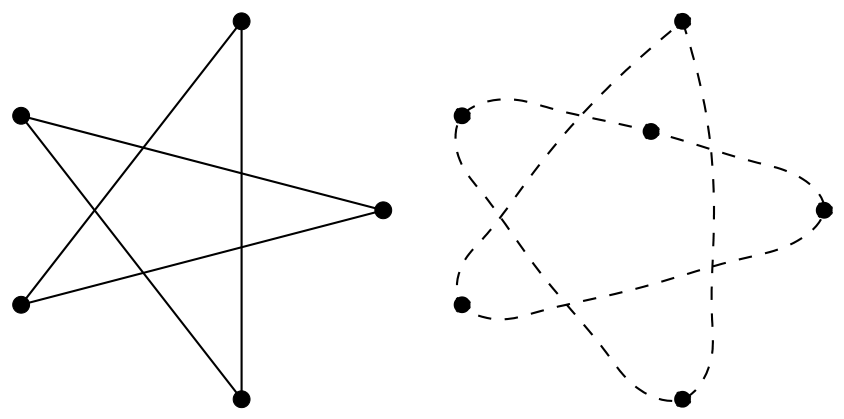
\includegraphics[width=0.5\textwidth]{fig12-pentagram.png}
  \caption{$\scrF(\Sigma_2)$ 的生成元与一个全纯六边形（原文 Figure~11，第 37 页）。\label{Fig:BalancedSphere}}
\end{figure}

选择 $\gamma_i$ 作为分裂生成元的动机来自 Seidel 的观察 \cite{Seidel:HMSgenus2}：
\[
\oplus_{i,j} HF^*(\gamma_i, \gamma_j) \ \cong \ \Lambda^*(V) \rtimes \bZ_{5}
\]
其中 $V$ 是三维向量空间。于是 $A_{\infty}$-结构可以借助第 \ref{Subsec:FiniteDeterminacy} 节的工具来处理（在存在有限群作用的情形下，这些工具有直接的等变版本），即以多向量场（polyvector field）来描述。直接计算表明，$A_{\infty}$-结构由一对 $(W,\eta)$ 给出，其中包含一个形式函数与一个形式 2-形式，满足
\[
W=z_1z_2z_3 + z_1^{5} + z_2^{5} + z_3^{5} + O(6)
\]
（我们忽略符号，它们可以通过在 Floer 复形中作适当的基变换来调整）。低阶非平凡系数来自高阶乘法 $\mu^3$ 与 $\mu^5$，它们由“明显”的全纯多边形确定：位于五角星各角处的三角形，或如图 \ref{Fig:BalancedSphere} 右侧所勾画边界的五边形（其到 $\bP^1$ 的投影在内五边形上以重数二覆盖）。在每种情形中，这些多边形都有一个额外的边界标记点，映射在该点处光滑但被限制在给定的某个拉格朗日上的一个圈上；在相应的四边形、六边形中，这表现为两条相邻的边界条件。由于 $W$ 在 $0$ 处有孤立奇点，它经形式变量替换等价于一个多项式，且事实上等价于其 $\leq 5$ 次 Taylor 级数。这以显式 $A_{\infty}$-代数上的模完整描述了 $\scrF(\Sigma_2)$ 的分裂闭包。

\subsection{四维环面\label{Sec:4torus}} 取 $\bK = \Lambda$。定理 \ref{Thm:LPelliptic} 的一个特殊情形（它更早即已为人所知）表明 $D^{\pi}\scrF(T^2) \simeq D^b(E)$，其中 $T^2$ 是方形辛环面，$E$ 是 Tate 曲线。Fukaya 范畴服从某种 Künneth 定理 \cite{AbouzaidSmith}；利用 Wehrheim--Woodward quilt 理论（的 $A_{\infty}$-精细版本），即第 \ref{Sec:Quilt} 节与 \eqref{Eqn:QuiltFunctor}，可以把 $D^{\pi}\scrF(T^2 \times T^2)$ 等同于 $D^{\pi}\scrF(T^2) \simeq D^b(E)$ 的自函子范畴。由此可知 $\scrF(T^4)$ 由四个拉格朗日二维环面 $l\times l, l\times m, m\times l, m\times m$ 分裂生成，且
\begin{equation} \label{Eqn:HMST4}
D^{\pi} \scrF(T^4) \simeq D^b(E\times E).
\end{equation}
\eqref{Eqn:HMST4} 对四维环面的辛拓扑有具体推论。设 $\phi: T^4 \rightarrow T^4$ 是一个在上同调上平凡作用的辛同胚。则它有定义良好的通量（flux），即：对任意 1-圈 $\gamma \in H_1(T^4)$，可取 2-链 $C_{\gamma}$ 使 $\partial C_{\gamma} = \gamma \cup \phi(\gamma)$，并考虑 $\int_{C_{\gamma}} \omega \in \bR / \bZ$，其中模去辛形式的周期便消除了 $C_{\gamma}$ 选取的不唯一性。

% [Tutor Note: Tate 曲线 $E$ 是 Novikov 域上的一条椭圆曲线，$D^{\pi}\scrF(T^2) \simeq D^b(E)$ 正是二维环面同调镜像对称的精确化。注意“方形”条件并非多余：$T^2$ 的辛面积与复结构参数决定 $E$ 的模参数（$j$-不变量），改变 $T^2$ 的复结构会改变镜像曲线。另一个易混点：通量是辛同胚同痕类的“平移部分”，Hamilton 同胚的通量恒为零。]

\begin{Proposition} 若 $\phi$ 的通量为零，则 $\phi$ 的 Hamilton 同痕类中任何具有非退化不动点的辛同胚都至少有 $16$ 个不动点。\end{Proposition}

\begin{proof}
$D^b(E\times E)$ 的自等价通过 Mukai、Orlov 与 Polishchuk 的工作已被完全理解，见 \cite{Orlov:abelian, Pol:weil}；那些在上同调上平凡作用的自等价，模去平移（shift），由张量以线丛以及 $E\times E$ 的平移生成。在辛侧，这些分别对应两类自等价：平移 $T^4$（具有非零通量），或给拉格朗日配备非平凡的局部系数（后者在空间层面、即 $T^4$ 的点上平凡作用）。因此，$\phi$ 与 $\scrF(T^4)$ 的恒等自等价（或 $T^4$ 的恒等辛同胚）有相同的 Floer 上同调，而后者恰为 $H^*(T^4)$。
\end{proof}

\subsection{二次超曲面}\label{Sec:Quadrics}

设 $X=Q \subset \bP^{2k+1}$ 为偶维二次超曲面。任何二次超曲面至多有一个结点，故 $X$ 含有一个在等痕意义下典范的拉格朗日球面 $L$：它是某个代数退化的消没圈，且这样的球面唯一。当 $k>0$ 时，它的极小 Maslov 数为 $2c_1(Q) > 2$，故落在零和分支 $\scrF(Q;0)\subset \scrF(Q)$ 中。

\begin{enumerate}
\item 设 $\scrX \rightarrow \bP^1$ 为二次超曲面族的一个 Lefschetz 铅笔的全空间：所有消没圈都同痕于固定的拉格朗日 $L$。容易验证，唯一的全纯截面来自对该铅笔底轨迹的爆破，因而在单个纤维中取值于 $Q \cap Q' \subset Q$，与第一 Chern 类成比例。于是命题 \ref{Prop:SpheresGenerate} 适用，$L$ 分裂生成 $\scrF(Q;0)$。
\item 或者考虑映射 $QH^*(Q;0) \rightarrow HF^*(L,L)$。两个空间秩均为 $2$，映射是幺的，故在 $0$ 次非平凡；又因 $[L] \neq 0 \in H_{2k}(Q)$，映射在 $2k$ 次非平凡（两边均按模 $4k$ 分次），故生成判据的第二个版本也适用。
\end{enumerate}

代数 $HF^*(L,L)$ 是半单的。由 $L$ 生成蕴含 $D^{\pi}\scrF(Q;0)$ 本质上是平凡的（等价于两个域上模之和，即向量空间对），见 \cite{Smith:HFQuadrics}。任何单连通的拉格朗日 $K \subset Q$ 都定义这样一个模，其自同态代数一方面是 $HF^*(K,K)$，另一方面是两个矩阵代数之和。

由于 $N_{min}(K) = 4k$，命题 \ref{Lem:Oh} 的 pearl 模型表明 Oh 谱序列按分次理由坍塌，且加性地有 $HF^*(K,K) \cong H^*(K)$。一个相当简单的代数几何计算 \cite{Beauville} 表明，量子上同调 $QH^*(Q)$ 含有一个 $2k$ 次的可逆元 $a$。由于 $\mathcal{CO}^0$ 是幺环同态，与 $\mathcal{CO}^0(a)$ 作积定义了（$\bZ/4k$-分次群）$HF^*(K,K)$ 的一个自同构；按命题 \ref{Lem:Oh} 的证明中提到的乘法 pearl 模型，该自同构由与 $a|_K$ 的经典杯积以及次数 $\leq 2k-N_{min}(K) = -2k$ 的修正给出。由此可知 $H^*(K)$ 在次数 $0<\ast< 2k$ 上消失，故 $K$ 是同调球面。又因 $H^*(K)$ 是两个矩阵代数之和，它必是两个一维如此代数之和，故 $K$ 定义的模与 $L$ 相同。于是 $K$ 在 $\scrF(Q;0)$ 中同构于 $L$，从而 $K \cap L \neq \emptyset$；特别地，任意两个单连通拉格朗日都不能经 Hamilton 同痕彼此移开。

% [Tutor Note: 这一段分次极易错位：$Q\subset\bP^{2k+1}$ 的复维数是 $2k$，$HF^*$ 是模 $4k$ 分次的（分次周期来自 $2c_1(Q)$），而 $QH^*$ 也是模 $4k$ 分次。文中“$[L]\neq 0\in H_{2k}$ 故映射在 $2k$ 次非平凡”依赖两侧分次约定的对齐；若套用通常的 $\bZ$-分次，$2k$ 会被误认为 $k$。]

任意 $Q$ 的辛同胚在 $\Auteq(\scrF(Q;0)) \cong \bZ_2$ 中都与恒等或与 Dehn 扭转 $\tau_L$ 重合，后者交换 $HF^*(L,L)$ 的两个幂等分支。由于二次曲面的粗模空间 $\EuScript{Q}$ 有基本群 $\bZ_2$，这意味着问题 \ref{Question:Monodromy} 中的映射在此情形是单射。

\subsection{环簇 Fano 簇} 设 $X$ 是环簇 Fano 簇，矩映射为 $\mu: X \rightarrow \frak{t}^*$，矩像为 $\Delta$。以矩映射的纤维为边界的 Maslov 2 圆盘由矩多面体 $\Delta$ 的余维一的面（facets）逐一枚举，这些计数可以组装成一个 Laurent 多项式 $W: \mathrm{int}(\Delta) \rightarrow \Lambda$，其单项式项由 $\Delta$ 各面的法向量决定，见 \cite{Cho,Cho-Oh}。（这个记号反映了如下事实：它契合第 \ref{Sec:Mirror} 节顺带提到的势函数一般图景。除子 $D$ 是 $X$ 的环簇边界，矩映射给出 $X\backslash D$ 的拉格朗日纤维化，而镜像 $\Cech{U} \cong (\bC^*)^n$。对 $\bP^2$，$W(x,y) = x+y+\lambda/xy$。）例 \ref{Ex:ToricFibre} 蕴含：矩映射的给定纤维的 Floer 上同调在某个局部系数下非平凡（即 $\partial_1 = 0$），当且仅当矩多面体的相应点是 $W$ 的临界值。

% [Tutor Note: 请牢牢记住“矩多面体的余维一面 $\leftrightarrow$ Maslov 2 圆盘类”这部字典：每个面贡献一个以矩映射纤维为边界的圆盘类，其（虚拟）计数给出 $W$ 中相应单项式的系数；而 $W$ 的临界点正对应那些可配上局部系数使 $\partial_1=0$ 的纤维（例 \ref{Ex:ToricFibre}）。这正是环簇镜像对称中 Landau--Ginzburg 势的辛侧来源。]

设 $X$ 的复维数为偶数 $n=2k$，且量子积 $\ast c_1(X)$ 的谱是单的，于是 $QH^*(X) = \oplus_{\lambda} QH^*(X;\lambda)$ 分解为域之和。此时存在 $\mathrm{rk}(QH^*(X))$ 个不同的局部系数 $\xi_j \rightarrow L$，定义在重心 $b\in\Delta$ 上方的环簇纤维 $L$ 上，使得 $HF^*(\xi_j, \xi_j)$ 非零；事实上在每种情形它都是 Clifford 代数（参见 \cite{Cho-Oh, FO3:toric, RitterSmith}）。对象 $(\xi_j \rightarrow L)$ 分裂为两两同构（至平移）的幂等元之和；偶维 Clifford 代数是矩阵代数，而闭-开弦映射
\[
QH^*(X;\lambda_j) \longrightarrow \bK \subset HH^*(Cl_n, Cl_n) 
\]
是到任一给定幂等分支的自同态子代数上的同构，因为该映射是幺的且两侧秩均为 1。定理 \ref{Thm:Generation} 蕴含 Fukaya 范畴由 $(L,\xi_j)$ 分裂生成，因此任何满足 $HF(K,K)\neq 0$ 的拉格朗日 $K$ 必与 $\mu^{-1}(b)$ 相交。

\subsection{四次曲面\label{Sec:K3}} 设 $Q= \{z_0^4+\cdots + z_3^4 = 0\}$ 为四次 $K3$ 曲面。由
\begin{equation}\label{pencil}
\lambda(z_0^4+ \cdots z_3^4) + z_0z_1z_2z_3
\end{equation}
定义的四次曲线铅笔在 $\lambda = 0$ 处的纤维之外是 Lefschetz 的，而 $\lambda = 0$ 处的纤维是坐标超平面之并。该铅笔有 $64$ 个结点纤维，由此得到 $Q$ 中一族 $64$ 个拉格朗日球面 $V_i$。以这些球面作正 Dehn 扭转的词通过一个平移作用在 $\scrF(Q)$ 上 \cite{Seidel:HMSquartic}；由命题 \ref{Prop:SpheresGenerate} 的一个变体可知这些球面分裂生成（此时 \eqref{eqn:concatenate} 中的映射因分次理由为零）。利用情形的对称性，Seidel 证明了
\[
\scrA(Q) \, = \, \oplus_{i,j} HF^*(V_i, V_j) \, \cong \, \Lambda(W) \rtimes \Gamma_{64}
\]
其中 $W$ 是四维复向量空间，$\Gamma_{64} \subset H \subset SL(W)$ 是 $SL(W)$ 的极大环面 $H$ 中由阶为 $4$ 的元素构成的有限子群。Hochschild 上同调 $HH^*(\Lambda(W)\rtimes \Gamma_{64})$ 含有由等变多向量场构成的和分支 $HH^*(\Lambda(W))^{\Gamma_{64}}$。对应于非弯曲形变（此时拉格朗日保持无障碍）的子群在 $2$ 次秩为 $7$，且存在\emph{唯一}一个在 $GL(W)$ 的 $\bZ_4$-子群（循环置换各坐标）下不变的类。该对称性保持铅笔 \eqref{pencil}，且 $\scrF(Q)$ 上的 $A_{\infty}$-结构可以取为此意义下不变的。这意味着在 Novikov 参数的任意给定阶，相关系数在差一个标量意义下唯一（由不变多项式 $y_0y_1y_2y_3$ 张成，其中 $y_i$ 是 $W^*$ 上的坐标）。结论是：$\scrA(Q)$ 上存在唯一的 $\bZ_4$-等变非形式 $A_{\infty}$-结构（至规范等价）。Seidel 验证了非形式性 \cite{Seidel:HMSquartic}，从而确定了 $D^{\pi}\scrF(Q)$ 的拟同构类。

在本例与此前考虑的亏格 2 曲线两种情形中，外代数的出现都颇为神奇。有一个更概念化的解释 \cite{Seidel:HMSgenus2, Sheridan}，它来自一个典范的浸入拉格朗日 $P \subset \bP^n\backslash \{(n+2) \, \mathrm{hyperplanes}\}$：其 Floer 上同调为外代数，而圆圈族 $\{\gamma_i\} \subset \Sigma_2$ 或球面族 $\{V_i\} \subset Q$ 则作为 $P$ 在射影空间的某个分歧覆盖下的全原像出现。$P$ 的构造又受到与镜像对称 SYZ 观点相关的想法启发。

% [Tutor Note: 此处“分次理由为零”指的是 $\eqref{eqn:concatenate}$ 中的闭-开弦型映射按次数不可能非零：消没球面 $V_i$ 的 Maslov 数与相关上同调类次数相差一个非零的量，故该映射只能是零映射。这是“正 Dehn 扭转的词只引起平移”这一结论能推出分裂生成的另一处关键分次计算。]

% [Tutor Note: 结论 $D^{\pi}\scrF(Q)\simeq D^b(Q)$（四次 K3 的同调镜像对称）依赖三个要素的汇合：(i) 64 个消没球面分裂生成；(ii) Hochschild 上同调中 $\bZ_4$-不变的非弯曲形变类唯一，从而 $A_\infty$-结构非形式且唯一；(iii) Seidel 对非形式性的显式验证。核对时注意 $\Gamma_{64}$ 是 $SL(W)$ 极大环面的 4 阶元素子群（阶 64），不是整个 $\bZ_4^3$。]

\begin{Notes} 关于 $T^2$，见 \cite{PolishchukZaslow, PZ2, LekiliPerutz, LekiliPerutz2}。关于超势与环簇，见 \cite{Auroux:slag, Cho, Cho-Oh, FO3:toric, RitterSmith, Woodward}。关于高亏格曲面、Calabi--Yau 或 Fano 超曲面以及某些完全交的 Fukaya 范畴，见 \cite{Efimov, Sheridan2, Sheridan3, Smith:HFQuadrics}。
\end{Notes}
